\documentclass[letterpaper,twocolumn,10pt]{article}
\usepackage{usenix-2020-09}

\usepackage{graphicx}
\usepackage[caption=false,font=footnotesize]{subfig}
\usepackage{booktabs}
\usepackage{tabularx}
\usepackage{array}
\usepackage{enumitem}
\usepackage{amsmath}
\usepackage{listings}
\usepackage{xspace}

\newcommand{\system}{QUASAR\xspace}
\newcommand{\dogi}{DOGI\xspace}
\newcommand{\midas}{MiDAS\xspace}
\newcommand{\sepbit}{SepBIT\xspace}
\newcommand{\zns}{ZNS\xspace}
\newcommand{\pqc}{PQC\xspace}
\newcommand{\etal}{et al.\xspace}

\newcolumntype{Y}{>{\raggedright\arraybackslash}X}
\newcolumntype{R}{>{\raggedleft\arraybackslash}X}

\lstset{
  basicstyle=\ttfamily\footnotesize,
  columns=fullflexible,
  frame=single,
  breaklines=true,
  xleftmargin=0.5em,
  xrightmargin=0.5em
}

\date{}
\title{\Large \bf \system: Cryptographic Intent-Aware Zoned Storage for Post-Quantum Workloads}
\author{Anonymous Submission}

\begin{document}
\maketitle

\begin{abstract}
Post-quantum services such as TLS terminators, KMS deployments, and audit systems write not only payload and logs, but also KEM artifacts, session-derived recovery records, key-wrap records, certificate metadata, and signatures whose lifetimes follow sessions, key epochs, rotations, and erase policy.
Zoned Namespace SSDs expose append and reset primitives that can exploit lifetime structure, but \dogi, \midas, and \sepbit infer lifetime from LBA locality, frequency, and previous invalidations, which do not encode the protocol event that kills a post-quantum secret.
This paper presents \system, a cryptographic intent-aware placement architecture that adds a 32-byte lifecycle hint to the write path, preserves history-based placement for ordinary payload, and packs short-lived post-quantum objects by death cohort so epoch close can reset eligible secret-bearing zones.
On an actual WD ZN540-class \zns SSD, a same-path replay over six DOGI-style workload axes completes 72 policy rows with no failures; \dogi-style placement leaves 99,834 stale secret blocks, while \system-\dogi hybrid leaves zero and reduces GC by 83.0\%, and FAST-style Sysbench plus dynamic Exchange-, Varmail-, and Alibaba-like pressure traces show 92.3--99.9\% GC reduction while preserving zero stale-secret exposure.
\end{abstract}

\section{Introduction}

Post-quantum cryptography is moving from a standards problem to a systems problem.  Once secure services adopt ML-KEM, ML-DSA, and related post-quantum mechanisms, the write path of a TLS terminator, key-management service, or signed logging system begins to carry more than application payload.  It also carries KEM ciphertexts, encapsulation metadata, session secrets, key-wrap records, certificate metadata, and signatures.  These objects are not all alike: some are append-only audit records, some are public metadata, and some are short-lived secrets whose lifetime ends at session close, epoch advance, or key rotation.

Zoned Namespace SSDs are a natural substrate for such services because they expose the structure that log-structured systems already exploit: data is appended into zones and reclaimed by resetting whole zones.  The placement problem is therefore crucial.  If objects that die together are placed together, a zone reset can reclaim space with little or no valid-block copying.  If short-lived and long-lived objects are mixed, the host must either copy residual live blocks during GC or leave expired data in place until a future cleaner selects the zone.  Recent \zns and log-structured placement systems, including \sepbit, \midas, and \dogi, attack this problem by inferring block lifetime from storage-visible history such as LBA, frequency, age, segment behavior, and prior invalidation time~\cite{sepbit,midas,dogi}.

The central mismatch in post-quantum workloads is that the lifetime of cryptographic artifacts is often not hidden at all.  The application or cryptographic runtime already knows that a session secret will die at session close, that a KMS envelope belongs to an epoch, and that a certificate object follows a rotation policy.  The storage device does not see this state.  From the perspective of a history-based placement system, a KEM artifact may look like another small write near a hot payload record.  From the perspective of the protocol, it belongs to a death cohort: a set of objects that become invalid together when the cryptographic state advances.

\begin{figure*}[t]
\centering
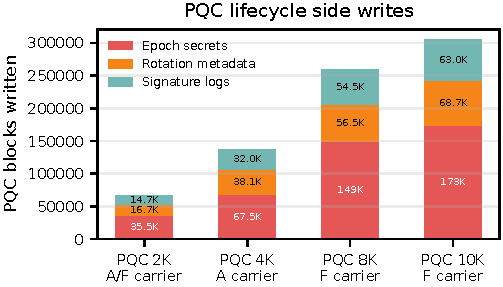
\includegraphics[width=0.68\textwidth]{../artifacts/figures/fast-style/fig1-intro-pressure.pdf}
\caption{Actual-\zns YCSB pressure with all history-based baselines.  The low-pressure row is intentionally a negative WAF control, while higher PQC overlays create GC pressure.  FIFO, \sepbit-style, \midas-style, and \dogi-style placement all leave expired secret blocks because they cannot see protocol death cohorts; \system-\dogi keeps secret cohorts reset-eligible and removes the exposure on the same rows.}
\label{fig:intro-ycsb}
\end{figure*}

\begin{table*}[t]
\centering
\caption{The paper's core gap.  Existing history-based placement systems observe storage history; \system observes the small lifecycle signal that defines post-quantum death cohorts.}
\label{tab:intro-gap}
\footnotesize
\begin{tabularx}{\textwidth}{lYYYY}
\toprule
\textbf{Policy} & \textbf{Main signal} & \textbf{Strength} & \textbf{PQC blind spot} & \textbf{Consequence} \\
\midrule
\sepbit-style & Write/invalidation history and group separation & Simple hot/cold-style lifetime grouping & Session close and key rotation are not encoded in history & Expired secrets remain mixed with payload or metadata. \\
\midas-style & Adaptive groups from historical invalidation patterns & Can keep WAF low on stable workloads & Stable storage history can hide protocol-driven burst invalidation & WAF may look good while stale secrets remain. \\
\dogi-style & Hybrid lifetime prediction and adaptive group organization & Strong general-purpose learned placement & MLP features do not include cryptographic epoch or intent & Pays prediction cost and still misses death cohorts. \\
\system-\dogi hybrid & DOGI-like payload placement plus cryptographic lifecycle hints & Keeps history placement where it is useful and adds semantic placement for secrets & Requires correct and conservative hint handling & Makes secret-bearing zones reset-eligible at epoch boundaries. \\
\bottomrule
\end{tabularx}
\end{table*}

Table~\ref{tab:intro-gap} gives the first-order distinction.  The point is not that learned placement is useless.  \dogi is designed for the regime where lifetime must be inferred from noisy storage behavior, and our own non-PQC controls preserve that advantage.  The point is that post-quantum metadata introduces a different regime: the lifetime boundary is a semantic event defined above the block layer.  Predicting this boundary from LBA and frequency is the wrong interface when a small lifecycle label can expose it directly.

This paper proposes \system, a cryptographic intent-aware \zns placement architecture.  \system follows one design rule: place data by when the cryptographic protocol will kill it, not by how the storage device has seen it before.  Each write carries a compact hint containing intent class, expiration class, security class, epoch, cohort identifier, and size.  The allocator maps short-lived secrets and KEM artifacts to epoch-secret zone families, maps rotation metadata to rotation families, keeps append-only signatures separate, and leaves ordinary payload on a history-based fallback.  The deployable default is a hybrid: \dogi-style placement remains responsible for payload locality, while \system handles the death cohorts that \dogi cannot observe.

The design also changes the security story of \zns placement.  Zone reset by itself is not a universal physical erase primitive, and we do not claim otherwise.  However, if expired secret bytes are scattered across mixed zones, the host cannot even issue a targeted reset or sanitize action without risking live data.  \system aligns secret lifetime with zone reset eligibility.  When the device or deployment provides hardware crypto-erase or sanitize semantics, the epoch manager can trigger that command at the protocol boundary; otherwise, \system still reduces the stale-secret exposure window by avoiding mixed secret zones.

Our evaluation follows the structure of the DOGI/FAST workload axis rather than inventing a clean PQC-only trace.  We use six DOGI-style workload families, YCSB-A/F pressure traces, dynamic Exchange-, Varmail-, and Alibaba-like pressure traces, and a FAST-style Sysbench-OLTP stressor.  We explicitly separate easy negative controls from WAF-pressure results.  On the actual \zns path, the six-axis fairness matrix completes 72 rows with no failed policy runs.  In that matrix, \dogi-style placement already has WAF near 1.0, but it leaves 99,834 stale secret blocks and issues no semantic physical resets.  \system-\dogi hybrid removes all stale secret blocks, issues 98 semantic resets, and reduces GC blocks by 83.0\%.  Under Sysbench pressure, the hybrid reduces \dogi-style GC blocks by 94.6\% and removes 38,438 stale secret blocks.  Under dynamic service pressure, it reduces GC by 92.3--99.9\% while keeping stale secret blocks at zero.

This paper makes the following contributions:

\begin{itemize}[leftmargin=*]
\item It identifies death cohorts as the missing placement unit for post-quantum storage workloads.  Unlike hotness or LBA locality, a death cohort is defined by cryptographic protocol state.
\item It presents \system, a \zns allocation architecture that uses a small lifecycle hint to separate short-lived secrets, rotation metadata, append-only signatures, and payload.
\item It implements a trace-driven and actual-\zns evaluation path with FIFO, \sepbit-style, \midas-style, \dogi-style, \system, and \system-\dogi hybrid policies.
\item It shows that the strongest claim is not universal WAF dominance.  Instead, \system exposes a semantic lifetime signal, removes stale-secret exposure across PQC overlays, and reduces WAF/GC when zone pressure makes mixed cohorts expensive.
\end{itemize}

\section{Background}

\subsection{ZNS Placement and Write Amplification}

\zns SSDs expose a storage interface in which each zone is written sequentially and later reset as a unit~\cite{zns}.  This interface removes part of the hidden device FTL policy and gives the host more control over placement.  The benefit depends on grouping objects with compatible lifetimes.  When a zone contains only expired objects, reset is cheap.  When a zone also contains live objects, the host must copy those valid blocks elsewhere before reset, increasing write amplification factor (WAF).

Prior placement systems therefore focus on predicting block invalidation time.  \sepbit separates data using historical invalidation behavior.  \midas adapts group configuration to workload patterns.  \dogi combines hot filtering, learned invalidation-time prediction, GC relocation policy, and dynamic group organization.  The DOGI paper evaluates both static-skew workloads such as FIO Zipf and YCSB-A/F and dynamic workloads such as Varmail, Alibaba, and Exchange~\cite{dogi}.  This is the right baseline family for \system because these systems represent the strongest storage-history approach.

\subsection{Post-Quantum Object Lifetimes}

Post-quantum workloads introduce a different kind of lifetime signal.  A KEM artifact or ephemeral secret is not short-lived because it has a particular LBA pattern; it is short-lived because the cryptographic protocol invalidates it.  A signature log may be append-only and long-lived, while a KMS envelope may die when an epoch closes.  A certificate metadata object may follow a rotation period rather than a session boundary.  These differences exist within the same service and often within the same burst of I/O.

\begin{table}[t]
\centering
\caption{Post-quantum objects have different lifetime and security behavior even when they are generated by the same service.}
\label{tab:pqc-objects}
\footnotesize
\begin{tabularx}{\columnwidth}{lYY}
\toprule
\textbf{Object} & \textbf{Lifetime driver} & \textbf{Placement implication} \\
\midrule
KEM artifact & Session or epoch close & Group by epoch; reset quickly. \\
Ephemeral secret & Session close & Isolate from payload and logs. \\
KMS envelope & Key epoch & Pack with same epoch family. \\
Certificate metadata & Rotation policy & Use rotation-zone family. \\
Signature log & Retention policy & Append-only placement. \\
Payload & Application update pattern & Use history-based fallback. \\
\bottomrule
\end{tabularx}
\end{table}

Table~\ref{tab:pqc-objects} gives the placement consequence.  A single hotness label cannot safely place these objects because two objects with similar write frequency may have opposite reclaim requirements.  Conversely, two objects with different LBAs and different sizes may be ideal zone neighbors if they die at the same epoch boundary.

\subsection{Claim Boundary}

\system is not an oracle.  It does not receive a future deletion timestamp for every object, and it does not assume that every hint is perfect.  The hint expresses lifecycle class and epoch membership, not secret key material.  Correctness is protected by a conservative epoch manager: a zone family is reset only after the manager confirms that all objects in that family have expired or have been safely migrated.

The security claim is also scoped.  Zone reset makes a zone reusable and can reduce exposure, but physical sanitization is device-dependent.  Our physical device advertises crypto-erase and block-erase sanitize support, and the crypto-erase sanitize command path has been executed successfully.  Nevertheless, the default claim is reset eligibility and exposure-window reduction.  A physical erase claim requires issuing sanitize or equivalent hardware crypto-erase semantics at epoch boundaries.

\section{Motivation}

\subsection{History Signals Do Not Encode Death Cohorts}

History-based placement asks: what did this block look like before?  \dogi-style policies observe LBA, previous LBA, access interval, segment frequency, and prior placement state.  These features are meaningful for ordinary payload updates because they capture hotness and locality.  A post-quantum secret asks a different question: which objects will die together when the protocol state advances?  The answer requires at least intent and epoch.

This distinction creates two failure modes.  The first is semantic: the baseline leaves expired secret blocks in zones that are not safely resettable because the zone also contains payload or long-lived metadata.  The second is performance: under sufficient free-zone pressure, mixed death cohorts force valid-block migration and raise WAF.  The first failure can appear even when WAF is near 1.0; the second appears only in harder pressure workloads.

\begin{figure}[!t]
\centering

\includegraphics[width=0.62\columnwidth]{../artifacts/figures/fast-style/fig2-motivation-semantic-gap-legend.pdf}\\[-0.4em]
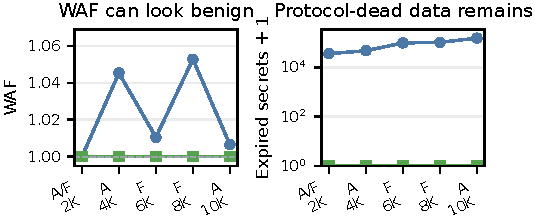
\includegraphics[width=0.98\columnwidth]{../artifacts/figures/fast-style/fig2-motivation-semantic-gap.pdf}
\caption{Motivation diagnostic: WAF is not enough to expose the PQC failure mode.  \dogi-style placement can look benign on storage-visible WAF while still stranding expired PQC secrets; \system-\dogi keeps payload on history placement but routes lifecycle objects by death cohort.}
\label{fig:motivation-semantic-gap}
\end{figure}

Figure~\ref{fig:motivation-semantic-gap} shows the diagnostic reason this paper does not use WAF alone as the motivation.  On DOGI-compatible YCSB carriers, \dogi-style placement often keeps physical WAF close to 1.0 because the payload locality signal is still useful.  At the same time, expired PQC secrets remain stranded because the storage-visible history does not encode epoch close.  \system-\dogi removes those protocol-dead secrets.  It routes only lifecycle objects through the death-cohort path.

\subsection{Easy Workloads Are Not Enough}

A clean PQC-only epoch trace makes \system look too good and is not a fair test of \dogi.  Our evaluation therefore treats such traces as sanity checks only.  The hard tests keep DOGI's normal locality signals and then add realistic PQC lifecycle writes.  Concretely, the workload matrix contains: DOGI-style six-axis fairness, YCSB-A/F pressure, FAST-style Sysbench pressure, dynamic service pressure, and QUASAR-hostile robustness.

\subsection{The Upper Bound Gives Design Requirements}

DOGI uses NoDaP to turn an oracle gap into design requirements.  \system uses a narrower epoch upper bound for the same diagnostic purpose: by giving the oracle exact PQC death cohorts, we test whether the missing signal is protocol lifetime rather than another storage-history feature.

The upper bound yields three requirements.  First, the placement path must expose protocol lifetime because LBA, frequency, and prior invalidations do not encode session close or key rotation.  Second, exact cohort placement must be budgeted because a sparse epoch per zone can trade WAF for poor utilization and too many active families.  Third, reset must be conservative because a wrong hint can hurt placement quality but must not discard live data.  These requirements lead directly to \system's lifecycle hint, admission/open-zone policy, and epoch-confirmed reclaim path.

The actual-\zns results later separate these failure modes.  In the six-axis fairness matrix, \dogi-style placement has WAF near 1.0 but leaves 99,834 stale secret blocks.  In harder YCSB, Sysbench, Exchange, Varmail, and Alibaba-like rows, history-based placement pays positive GC while leaving stale secrets; the hybrid keeps payload on history placement and moves PQC secrets into resettable cohorts.

\subsection{The Desired Design Shape}

The design requirement is therefore not ``replace DOGI everywhere.''  A pure semantic allocator can be worse for ordinary payload.  The desired system uses history where history is the right signal and cryptographic intent where history is blind: DOGI-like placement for payload, \system zone families for PQC lifecycle objects, and conservative fallback for unreliable hints.

\section{Design}

\subsection{Overview}

\system is a host-side placement layer for \zns devices.  Figure~\ref{fig:architecture} shows the data path.  Applications or cryptographic libraries produce lifecycle labels when they create PQC artifacts.  These labels are attached to writes as \texttt{quasar\_hint}.  The allocator maps each write to a zone family.  An epoch manager tracks which families are eligible for reset, migration, or fallback GC.  Payload writes continue to use a history-based fallback, so the system does not discard the strengths of \dogi-style placement.

\begin{figure*}[t]
\centering
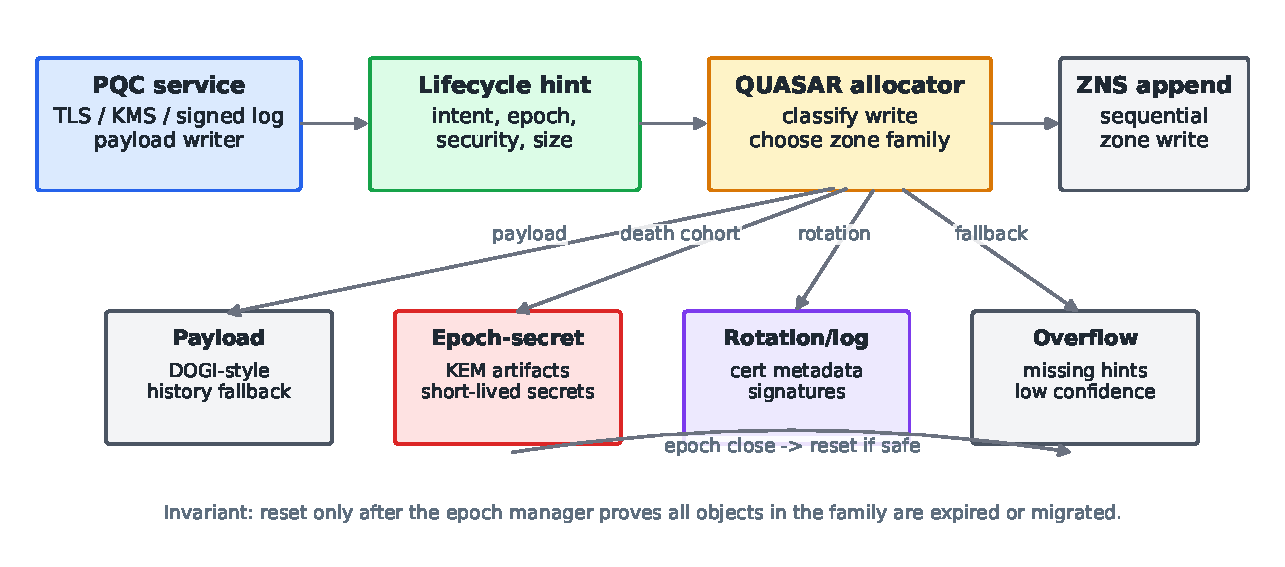
\includegraphics[width=0.86\textwidth]{../artifacts/figures/paper/quasar-architecture.pdf}
\caption{\system architecture.  The storage path receives lifecycle labels, not secret material.  Payload remains on a history-based fallback, while PQC secrets, rotation metadata, and uncertain writes are routed to separate zone families.  The epoch manager resets or sanitizes a family only after proving that all objects in the family are expired or migrated.}
\label{fig:architecture}
\end{figure*}

\subsection{Design Requirements}

\system follows the three requirements from Motivation.  Lifecycle labels expose protocol lifetime and route PQC objects to death-cohort zone families while payload stays on \dogi-style fallback.  Admission control budgets exact placement by reserving scarce exact families for high-security secrets and sending sparse or uncertain writes to bins or overflow.  Epoch-confirmed reclaim resets a family only after durable epoch close or residual migration; uncertain zones fall back to normal GC.  The evaluation checks these requirements with stale-secret exposure rows, pressure traces, multi-tenant stress, bad hints, and sanitize-boundary tests.

\subsection{Hint Schema}

The hint is intentionally small.  It contains only lifecycle metadata:

\begin{lstlisting}[language=C,caption={Minimal \system hint schema.},label={lst:hint}]
enum quasar_intent {
  QUASAR_PAYLOAD = 0,
  QUASAR_EPHEMERAL_SECRET = 1,
  QUASAR_KEM_ARTIFACT = 2,
  QUASAR_SIGNATURE_LOG = 3,
  QUASAR_CERT_METADATA = 4,
};

struct quasar_hint {
  uint16_t intent;
  uint16_t expire_class;
  uint32_t security_class;
  uint64_t epoch_id;
  uint64_t cohort_id;
  uint64_t size_bytes;
};
\end{lstlisting}

The fields are lifecycle labels, not cryptographic secrets.  \texttt{intent} separates secrets, KEM artifacts, signature logs, certificate metadata, and payload.  \texttt{epoch\_id} identifies the death cohort.  \texttt{security\_class} sets reset urgency and isolation.  \texttt{cohort\_id} is opaque to storage and can be a keyed hash, so raw session, tenant, or key identifiers need not cross the storage boundary.

\noindent\textbf{Trust boundary.}
\system assumes that high-priority lifecycle hints are emitted by trusted components such as the TLS terminator, KMS, logging service, or a privileged policy layer.  Untrusted tenants do not directly grant themselves exact secret-zone priority.  A deployment can enforce per-tenant exact-family quotas, tenant-local cohort namespaces, and admission limits before a hint reaches the allocator.  If provenance is missing or confidence is low, the write is routed to overflow and becomes a performance/exposure tradeoff rather than a correctness risk.

\subsection{Zone Families}

\system allocates writes into a small set of zone families:

\begin{table}[t]
\centering
\caption{\system zone families.  Each family maps a lifecycle class to a reclaim rule, separating short-lived secrets from payload and append-only logs.}
\label{tab:zone-family}
\footnotesize
\begin{tabularx}{\columnwidth}{lYY}
\toprule
\textbf{Family} & \textbf{Data} & \textbf{Reclaim rule} \\
\midrule
Epoch-secret & KEM artifacts, ephemeral secrets & Reset when epoch expires. \\
Rotation & Certificates, key metadata & Reset on rotation boundary. \\
Append-log & Signatures, audit records & Normal append-log reclaim. \\
Payload & Application payload & History-based fallback. \\
Overflow & Missing or low-confidence hints & Conservative GC or migration. \\
\bottomrule
\end{tabularx}
\end{table}

The key invariant is separation: the allocator keeps short-lived secrets out of long-lived payload and append-only log zones unless explicit pressure routes them through a conservative fallback.  This is the mechanism that turns protocol lifetime into reset eligibility.

\subsection{Allocation Procedure}

For each write, \system first classifies the object:

\begin{lstlisting}[caption={Zone-family decision rule.},label={lst:alloc}]
if intent in {EPHEMERAL_SECRET, KEM_ARTIFACT}:
    family = EPOCH_SECRET_ZONE(epoch_id, security_class)
elif intent == CERT_METADATA:
    family = ROTATION_ZONE(rotation_epoch(epoch_id))
elif intent == SIGNATURE_LOG:
    family = APPEND_LOG_ZONE
elif intent == PAYLOAD:
    family = DOGI_HISTORY_FALLBACK
else:
    family = OVERFLOW_ZONE
\end{lstlisting}

The allocator appends the write to the active zone for that family.  If the active zone lacks capacity, the zone is closed and a new zone is allocated.  When the active-zone budget is tight, \system preserves exact placement for secret data first, bins lower-risk KEM artifacts or sparse epochs second, and routes uncertain writes to overflow.  This priority order prevents a utilization-first policy from degenerating into arbitrary mixing.

\subsection{Admission Control and Open-Zone Budget}

Exact epoch placement is useful only when the device can afford the active families it creates.  Real \zns devices bound the number of open and active zones; the evaluated device exposes a limit of 13 for both open and active zone accounting in our robustness experiments.  \system therefore admits exact epoch-secret families only when the expected epoch bytes justify a dedicated zone and the active family count remains below the budget.

When a sparse or multi-tenant workload would exceed the budget, \system degrades in a fixed order.  It first keeps exact families for high-security secrets, then bins lower-risk or sparse cohorts by coarse epoch ranges, then routes low-confidence writes to overflow.  This policy makes the cost visible: exact placement maximizes exposure reduction, binning trades some exposure precision for zone budget, and overflow preserves correctness when the hint path is unreliable.

\begin{table}[t]
\centering
\caption{Main \system policy parameters.  These knobs expose the cost of exact placement: active-zone budget, sparse-epoch binning, residual migration, hint confidence, and tenant isolation are workload/device inputs, not hidden oracle information.}
\label{tab:params}
\footnotesize
\begin{tabularx}{\columnwidth}{lY}
\toprule
\textbf{Parameter} & \textbf{Role} \\
\midrule
Active-family budget & Caps concurrently open/active death-cohort families; robustness runs use the device-reported 13-zone budget. \\
Minimum epoch fill / bin width & Decides whether sparse epochs receive exact zones or coarse cohort bins. \\
Residual threshold / copy budget & Bounds live-byte migration before reset; strict mode raises this budget to force zero waiting. \\
Hint confidence & Sends missing, untrusted, or inconsistent hints to overflow instead of exact secret zones. \\
Tenant mode & Uses tenant-local bins and quotas when reset-time tenant mixing is not acceptable. \\
\bottomrule
\end{tabularx}
\end{table}

\subsection{Epoch Reclaim}

At epoch close, the epoch manager evaluates all zone families associated with that epoch:

\begin{lstlisting}[caption={Conservative epoch reclaim.},label={lst:reclaim}]
on epoch_expire(epoch_id):
  for zone in zones_owned_by(epoch_id):
    if live_bytes(zone) == 0:
      reset(zone)
    elif live_bytes(zone) <= residual_threshold:
      migrate_live_bytes(zone)
      reset(zone)
    else:
      downgrade_to_normal_gc(zone)
\end{lstlisting}

This rule makes wrong hints a performance problem rather than a correctness problem.  A family is reset only after the epoch manager confirms that every object in the family has expired or has been safely migrated.  If the system cannot prove safety after a crash or hint inconsistency, it routes the zone to normal GC.

\subsection{Crash and Recovery Invariant}

\system cannot keep epoch-to-zone ownership only in volatile memory.  Each zone family has durable metadata that records its family identifier, epoch, intent class, and reset generation.  After a crash, recovery scans this metadata, rebuilds the family-to-zone map, replays durable epoch-close records, and resets only zones whose epoch close is known to be durable.  Uncertain zones are downgraded to normal GC.  This conservative rule is central to the security story: a bad hint or incomplete recovery can reduce placement quality, but it must not cause a live object to be discarded.

\subsection{Deployment Modes}

The deployable design is not a single universal knob.  The default mode is \system-\dogi hybrid: history-based placement for payload and death-cohort placement for PQC secrets.  Tenant-isolation mode uses tenant-local bins when reset-time tenant mixing is unacceptable.  Strict-residual mode copies delayed-expiry stragglers to force zero final secret waiting.  Overflow mode handles missing or low-confidence hints.  These modes make the cost visible instead of pretending that perfect epoch alignment is free.

\section{Implementation}

\subsection{Trace and Replay Infrastructure}

We implemented \system as a trace-driven allocator and actual-\zns replay framework.  The trace format records writes, expirations, object identifiers, sizes, LBA-like payload location, intent, epoch, security class, tenant, and confidence.  The same trace is replayed through FIFO, \sepbit-style, \midas-style, \dogi-style, \system, and \system-\dogi hybrid policies.  This keeps timing and object lifetimes identical across policies.

The deployment hook is intentionally small: a TLS terminator, KMS, or logging component emits the 32-byte \texttt{quasar\_hint} when it writes a KEM artifact, ephemeral secret, certificate record, or signature log.  The hint can travel as request context in user-space replay or as file/extent metadata in a filesystem path; it does not carry key material.

The workload generators produce three classes of traces.  First, DOGI-paper-shaped traces mirror the workload axes described by DOGI: FIO Zipf, YCSB-A, YCSB-F, Varmail, Alibaba, and Exchange.  Second, pressure traces increase PQC density and reduce free-zone slack to force GC.  Third, hostile traces introduce missing hints, wrong epochs, tenant pressure, and stragglers.  The implementation also includes a real FIO iolog converter that maps benchmark-issued FIO writes into the same QUASAR JSONL schema before adding PQC lifecycle side writes.  We additionally ran a Sysbench/MySQL execution gate.  Full YCSB/JDBC or Sysbench block traces would strengthen external validity, but the scoped claim uses the DOGI/FAST-shaped physical pressure suites and exact external baseline runs as the paper-grade placement evidence.

\subsection{Baseline Implementations}

The same-path comparison implements FIFO, \sepbit-style, \midas-style, and \dogi-style policies in the replay framework.  These implementations are intentionally described as style-compatible baselines because they share the same physical packed-\zns path as \system.  The artifact set also contains exact public DOGI/MiDAS/SepBIT runs in their native environments.  We keep these exact runs separate from the same-path results because their units and internal segment models are not identical to the packed replay path.

\subsection{Physical ZNS Path}

The actual-\zns experiments use a Western Digital ZN540-class \zns NVMe SSD mounted with \texttt{zonefs}.  The replay writes zone files sequentially and issues reset-like truncation or helper operations according to the policy plan.  This path measures full-suite append/reset accounting, but it includes zonefs helper overhead.  We therefore report it as actual-\zns replay overhead, not as final production p99 latency.

To check the lower-overhead command path, we also implemented an xNVMe raw \zns latency probe.  The local xNVMe backend uses Linux NVMe ioctl synchronous commands.  It bypasses the zonefs helper path and completes 4,096 4KiB appends with p99 append latency of 26,064 ns.  This is not an SPDK poll-mode result, but it bounds the helper-path caveat.

\subsection{Security Capability Check}

The physical device reports sanitize capability with crypto-erase and block-erase support.  We executed an NVMe crypto-erase sanitize command on the device and observed successful completion in the sanitize log.  This validates the command path for hardware crypto-erase.  The evaluation keeps this separate from zone reset: \system makes secret-bearing zones eligible for reset and, when configured, for explicit sanitize or crypto-erase commands.

\section{Evaluation}

\subsection{Methodology}

The evaluation answers five questions:

\begin{enumerate}[leftmargin=*]
\item Does \system avoid relying on an easy PQC-only trace?
\item Does \system remove stale-secret exposure on DOGI-style workload axes?
\item Under pressure, does \system reduce WAF and GC relative to history-based placement?
\item What overhead does semantic placement introduce?
\item What security claim is supported by actual device capability?
\end{enumerate}

\noindent\textbf{Evaluation platform.}
We evaluate placement with trace-driven replay and an actual \zns device: a Western Digital ZN540-class NVMe SSD exposed as \texttt{/dev/nvme0n1} and mounted through \texttt{zonefs}.  The replay model uses 4KiB logical blocks and a 275,712-block zone capacity.  As in DOGI's methodology, the simulator/replay path gives broad policy coverage, while the physical path validates that the planned append/reset schedule executes on a zoned device.  Because the full-suite path includes zonefs helper overhead, we report its latency as overhead accounting rather than production SPDK p99 latency.

\noindent\textbf{Baselines.}
We compare against FIFO, \sepbit-style, \midas-style, and \dogi-style placement.  These are same-path policies in our simulator and actual-\zns replay.  We also keep exact public DOGI/MiDAS/SepBIT runs as separate evidence because their internal units are not directly interchangeable with our packed \zns replay.

\noindent\textbf{Workloads.}
The fairness matrix uses six DOGI-style axes: FIO Zipf, YCSB-A, YCSB-F, Varmail, Alibaba, and Exchange.  Headline WAF rows keep these locality signals and add PQC lifecycle side writes through high-ratio YCSB-A/F, FAST-style Sysbench-OLTP pressure, and dynamic Exchange/Varmail/Alibaba-like traces.  Pure PQC epoch streams are sanity checks, not headline evidence.  Hostile robustness uses tenant mixing, missing hints, wrong hints, and stragglers; real FIO iolog and Sysbench/MySQL gates check benchmark readiness.

\noindent\textbf{Metrics.}
We report WAF, GC write blocks, stale secret blocks, semantic physical reset count, secret bytes waiting for physical reset, zone utilization, live physical zones, append/reset latency, and C-level placement-decision overhead.  A stale secret block is an expired secret-class logical block in a family that is not safely reset- or sanitize-eligible because live data remains or epoch close is unproven.  Exposure artifacts report stale-secret block-seconds; physical tables use final and representative stale-block counts for auditability.  WAF alone is insufficient because a policy can keep WAF near 1.0 while leaving expired PQC secrets in mixed zones.
For example, the E4 exposure timeline records max stale-secret block-seconds of 69,391,500 for FIFO and \dogi-style placement, while \system remains at zero block-seconds and zero final stale-secret blocks.

\subsection{Workload Hardness}

The workload hardness rule is: DOGI-friendly first, PQC-hostile second.  A headline WAF/GC row must preserve storage-visible structure that helps history-based placement---hot/cold skew, overwrite locality, segment reuse, or phase changes---and then add PQC objects whose invalidation follows protocol state rather than LBA history.  Pure PQC-only traces, oracle-expiration traces, and low-pressure rows are sanity checks or exposure evidence.

The matrix passes all nine gates: fairness, negative controls, pressure rows, main-claim eligibility, and hostile robustness.  The artifact set has seven eligible YCSB pressure rows, nine YCSB baseline-complete rows, three dynamic eligible rows, and DB pressure eligibility.  Rows with WAF near 1.0 are interpreted as semantic exposure results; WAF/GC claims come only from rows where history-based policies pay positive GC or copied-live-block cost.

\subsection{Epoch Upper Bound}

DOGI uses NoDaP as an oracle-like target for lost lifetime information.  We use a narrower upper bound: an epoch oracle that sees exact death time at write time.  It is not deployable and is not counted as \system; it tests whether the workload is placeable once the protocol-lifetime signal exists.

On the mixed sanity trace, \dogi-style placement has WAF 1.791 and 484,967 GC blocks, \system has WAF 1.010 and 6,331 GC blocks, and the epoch oracle has WAF 1.000 and zero GC blocks.  On the stress-rekey trace, \dogi-style placement has WAF 2.031, \system has WAF 1.019, and the oracle has WAF 1.003.  These synthetic rows are bounds, not headline evidence: most of the gap comes from whether the allocator can observe the protocol lifetime boundary.

\begin{figure*}[t]
\centering
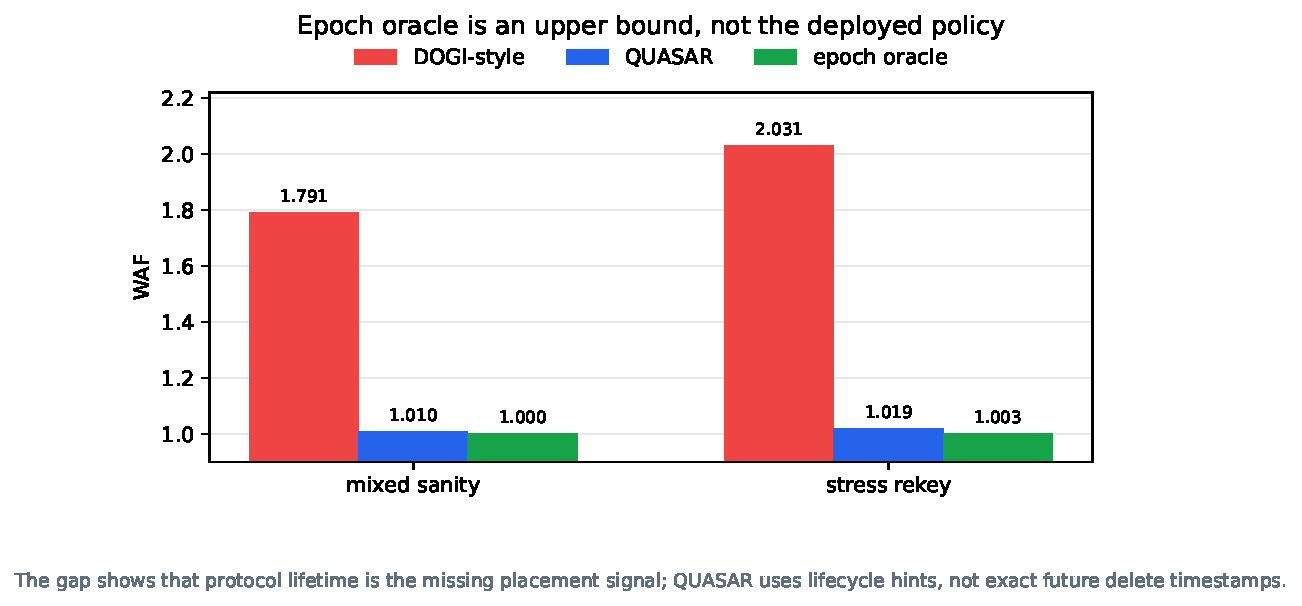
\includegraphics[width=0.72\textwidth]{../artifacts/figures/paper/epoch-upper-bound.pdf}
\caption{Epoch upper bound.  The epoch oracle is not a deployable baseline; it receives exact future death time.  Its role is to show that the WAF gap is largely a missing-lifetime-signal problem.  \system approaches the upper bound with lifecycle hints, while the paper's headline claims still come from harder physical-\zns pressure rows.}
\label{fig:epoch-upper-bound}
\end{figure*}

\subsection{DOGI-Favorable Control}

The non-PQC control verifies that the hybrid preserves history placement.  On the six DOGI-style axes with no PQC side writes, \dogi-style placement and the \system-\dogi hybrid produce the same WAF because payload stays on the history policy.  \dogi-style placement beats FIFO and pure \system on all six workloads, and no stale secret blocks exist.  This keeps the claim boundary clear: \system is not a replacement for learned placement when no cryptographic death-cohort signal exists.

\subsection{Same-Path Fairness Matrix}

The six-axis actual-\zns fairness matrix completes 72 rows with zero failures.  Table~\ref{tab:fairness} reports the aggregated policy results.  \dogi-style placement is already strong on WAF, which is expected on an easy fairness matrix.  However, it leaves 99,834 stale secret blocks and performs no semantic physical resets.  \system-\dogi hybrid leaves zero stale secret blocks, performs 98 semantic resets, and reduces GC blocks from 625 to 106.

\begin{table}[t]
\centering
\caption{Same-path actual-\zns fairness matrix over six DOGI-style axes at pqc2000.  The easy matrix keeps \dogi-style WAF near 1.0, but only \system-\dogi hybrid removes stale secrets while reducing GC.}
\label{tab:fairness}
\footnotesize
\begin{tabularx}{\columnwidth}{lRRRR}
\toprule
\textbf{Policy} & \textbf{WAF} & \textbf{GC} & \textbf{Stale secrets} & \textbf{Resets} \\
\midrule
FIFO & 1.0040 & 3,903 & 99,141 & 0 \\
\sepbit-style & 1.0023 & 2,241 & 99,822 & 0 \\
\midas-style & 1.0006 & 581 & 99,898 & 0 \\
\dogi-style & 1.0006 & 625 & 99,834 & 0 \\
\system & 1.0011 & 1,121 & 0 & 98 \\
\system-\dogi hybrid & 1.0001 & 106 & 0 & 98 \\
\bottomrule
\end{tabularx}
\end{table}

The WAF gain here is deliberately modest: 0.1\% relative to \dogi-style.  The row is a semantic result, not a performance headline: storage-history placement can have good WAF and still fail to make expired PQC secrets resettable.

\subsection{YCSB Pressure}

YCSB pressure creates the WAF/GC separation missing from easy p2000 rows.  Table~\ref{tab:ycsb} reports representative physical \zns replays.  \dogi-style placement pays 3,357--24,289 GC blocks and leaves 46,266--150,221 stale secret blocks.  The hybrid removes stale secret blocks in all rows and reduces GC to zero in these representative replays.

\begin{table*}[t]
\centering
\caption{Representative actual-\zns YCSB pressure replays.  These traces keep YCSB update locality while adding PQC lifecycle side writes, showing where pressure turns the semantic gap into measurable GC/WAF cost.}
\label{tab:ycsb}
\footnotesize
\begin{tabularx}{\textwidth}{lRRRRRRR}
\toprule
\textbf{Workload} & \textbf{DOGI WAF} & \textbf{Hybrid WAF} & \textbf{DOGI GC} & \textbf{Hybrid GC} & \textbf{DOGI stale} & \textbf{Hybrid stale} & \textbf{Hybrid resets} \\
\midrule
YCSB-A pqc4000 & 1.0454 & 1.0000 & 15,316 & 0 & 46,266 & 0 & 28 \\
YCSB-A pqc6000 & 1.0376 & 1.0000 & 15,308 & 0 & 76,950 & 0 & 28 \\
YCSB-A pqc10000 & 1.0066 & 1.0000 & 3,357 & 0 & 150,221 & 0 & 26 \\
YCSB-F pqc6000 & 1.0105 & 1.0000 & 4,166 & 0 & 96,050 & 0 & 28 \\
YCSB-F pqc8000 & 1.0528 & 1.0000 & 24,289 & 0 & 100,847 & 0 & 28 \\
YCSB-F pqc10000 & 1.0279 & 1.0000 & 13,741 & 0 & 144,901 & 0 & 26 \\
\bottomrule
\end{tabularx}
\end{table*}

The p10000 rows bound the WAF claim.  Dense YCSB overlays can keep \dogi-style WAF close to 1.0, yet the stale-secret gap remains large.  WAF improvement appears under pressure; exposure improvement appears across PQC overlays.

\subsection{Multi-Seed Ratio Sweep}

To check that the pressure result is not a single-seed artifact, we run a three-seed ratio sweep over the six DOGI-style workload families at 0\%, 5\%, and 20\% PQC overlay ratios, for 54 comparisons.  The hybrid matches \dogi-style at 0\% PQC, is WAF-negative at 5\% PQC (-1.1\% mean WAF, -12.4\% mean GC) while avoiding 2,342 stale secret blocks per seed, and becomes positive at 20\% PQC (5.0\% mean WAF and 38.3\% mean GC improvement) while avoiding 10,021 stale secret blocks per seed.  Thus low-ratio overlays are exposure evidence, not WAF wins; WAF/GC benefits appear once protocol-lifetime objects create enough placement pressure.

\subsection{DB and Dynamic-Service Pressure}

Table~\ref{tab:pressure} reports the harder Sysbench and dynamic service rows.  Sysbench is not a DOGI-paper workload; it is included as FAST-style DB pressure.  The hybrid reduces \dogi-style GC from 11,256 to 609 blocks and removes 38,438 stale secret blocks.  On Exchange-, Varmail-, and Alibaba-like dynamic traces, the hybrid reduces GC by 92.3--99.9\% and keeps stale secrets at zero.

\begin{figure*}[t]
\centering
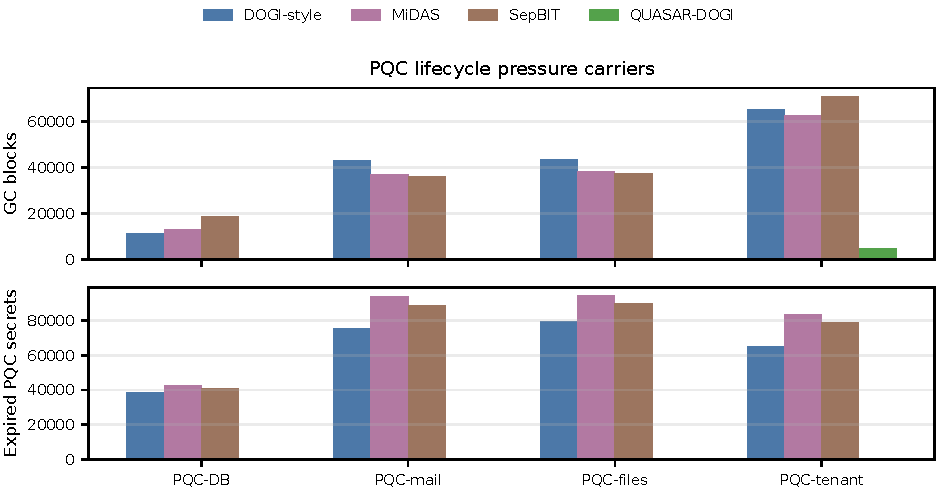
\includegraphics[width=0.88\textwidth]{../artifacts/figures/fast-style/fig2-pressure-breadth.pdf}
\caption{FAST-style pressure breadth.  Sysbench, Exchange, Varmail, and Alibaba-like rows keep storage-visible locality while adding PQC lifecycle objects.  History-based policies can still group payload, but they do not make expired secret cohorts reset-eligible; \system-\dogi cuts GC and stale-secret exposure on the same pressure axes.}
\label{fig:pressure-breadth}
\end{figure*}

\begin{table*}[t]
\centering
\caption{FAST-style DB and dynamic-service pressure.  Dynamic rows use DOGI-style workload families with high PQC overlays and tight logical-zone pressure; the hybrid preserves zero stale secrets while cutting GC.}
\label{tab:pressure}
\footnotesize
\begin{tabularx}{\textwidth}{lRRRRRRR}
\toprule
\textbf{Workload} & \textbf{DOGI WAF} & \textbf{Hybrid WAF} & \textbf{DOGI GC} & \textbf{Hybrid GC} & \textbf{DOGI stale} & \textbf{Hybrid stale} & \textbf{GC reduction} \\
\midrule
Sysbench-OLTP pressure & 1.0301 & 1.0016 & 11,256 & 609 & 38,438 & 0 & 94.6\% \\
Exchange-like pqc8000 & 1.0716 & 1.0000 & 43,006 & 22 & 75,422 & 0 & 99.9\% \\
Varmail-like pqc8000 & 1.0727 & 1.0003 & 43,227 & 175 & 79,600 & 0 & 99.6\% \\
Alibaba-like pqc8000 & 1.0974 & 1.0075 & 65,010 & 4,992 & 65,184 & 0 & 92.3\% \\
\bottomrule
\end{tabularx}
\end{table*}

These rows are the strongest performance evidence because all non-QUASAR baselines complete but pay visible GC and leave stale secrets.  They also show why the hybrid is the default deployable policy: payload placement remains history-based, while secrets are placed by protocol cohort.

\subsection{Component Ablation}

Table~\ref{tab:ablation} turns the upper-bound requirements into mechanism evidence.  History-only placement is the right first row because it gives \dogi-style placement all storage-visible signals but no protocol lifetime.  Adding lifecycle hints removes stale secrets, but pure semantic grouping can still leave GC cost on DB-like payload.  Adding the \dogi payload fallback removes that remaining cost.  Admission and residual migration are not free performance wins; they are boundary mechanisms for open-zone pressure and stragglers.  Figure~\ref{fig:component-ablation} shows the mechanism split visually, and Figure~\ref{fig:resource-overhead} visualizes the space and overhead controls.

\begin{figure*}[t]
\centering
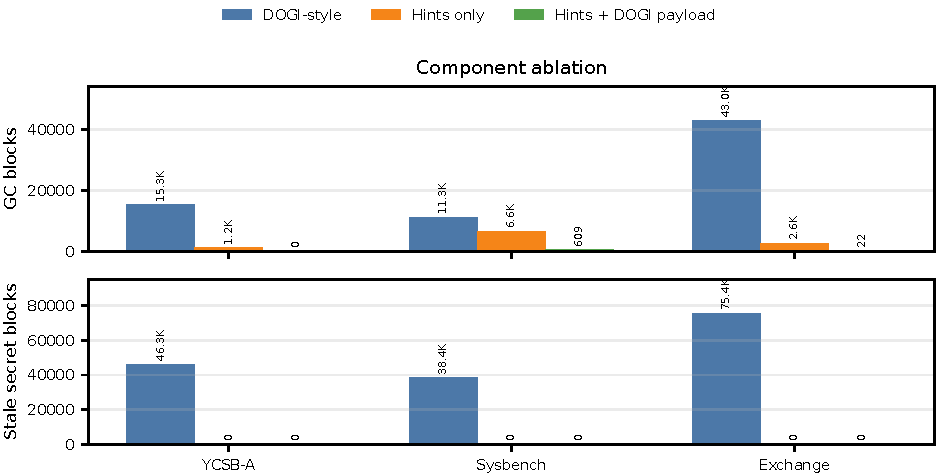
\includegraphics[width=0.88\textwidth]{../artifacts/figures/fast-style/fig3-component-ablation.pdf}
\caption{Component ablation.  A history-only \dogi-style policy sees storage history but misses death cohorts, so GC and stale-secret exposure remain.  Lifecycle hints remove exposure; adding \dogi-style payload fallback recovers payload placement and removes the remaining GC in the default hybrid.}
\label{fig:component-ablation}
\end{figure*}

\begin{table*}[t]
\centering
\caption{Component ablation from actual-\zns and pressure artifacts.  Lifecycle hints remove stale secrets, the \dogi payload fallback recovers payload GC behavior, and residual migration exposes the cost of strict zero-wait security.}
\label{tab:ablation}
\scriptsize
\begin{tabularx}{\textwidth}{lYYY}
\toprule
\textbf{Component} & \textbf{Evidence} & \textbf{Lesson} & \textbf{Decision} \\
\midrule
History only & DOGI YCSB-A p4000: GC 15,316, stale 46,266, resets 0. & History misses protocol death. & Do not place secrets by history alone. \\
Lifecycle hints & Pure \system: YCSB-A stale 0; Exchange stale 0. & Hints carry the missing signal. & Route PQC objects by death cohort. \\
Payload fallback & Hybrid cuts Sysbench GC 6,567$\rightarrow$609 and Exchange GC 2,610$\rightarrow$22. & Payload still needs history. & Keep \dogi fallback as default. \\
Admission & Exact hybrid wins 6 YCSB/Sysbench rows; adaptive wins 0. & Binning is not free. & Use adaptive only under pressure. \\
Residual & Stragglers: binning caps 13 zones but leaves 40,454 waiting; residual reaches 0 at WAF 1.7098. & Strict exposure has copy cost. & Expose low/strict profiles. \\
\bottomrule
\end{tabularx}
\end{table*}

\subsection{Exact Public Baseline Sanity Runs}

The main tables use same-path replay so FIFO, \sepbit-style, \midas-style, \dogi-style, \system, and the hybrid share trace timing, packed physical-\zns model, and reset accounting.  We also ran public baseline artifacts in their native environments.  Public DOGI completes Alibaba p8000 compact, selector-suite, and original-LBA runs with reported WAF 2.993, 2.804, and 3.212; public MiDAS completes compact FIO and PQC representatives with WA 1.000 and 1.250; public SepBIT completes a PQC pressure representative with WA 2.430.  These runs are sanity evidence, not apples-to-apples WAF numbers.  They sharpen the boundary: MiDAS is strong on at least one compact representative, so the claim rests on death-cohort exposure and same-path pressure evidence, not universal baseline collapse.

\subsection{Overhead}

\system adds semantic reset work, but its decision path is cheap.  In the actual-\zns overhead suite, the hybrid issues 318 more semantic reset operations than \dogi-style.  Zonefs-helper throughput is lower than \dogi-style by this accounting, but helper latency includes user-space append/truncate overhead.  In the C-level placement-decision benchmark, \dogi-style feature extraction plus a small MLP costs 2,397.8 ns/write, \system hint routing costs 16.8 ns/write, and the hybrid costs 1,178.8 ns/write.

The xNVMe probe provides a lower-overhead command-path sanity check: 4,096 4KiB zone appends complete with p99 latency of 26,064 ns and throughput of 181.79 MiB/s.  The probe is a Linux NVMe ioctl path, not SPDK poll-mode, so it is reported as a bound rather than a final production datapoint.

\begin{figure*}[t]
\centering
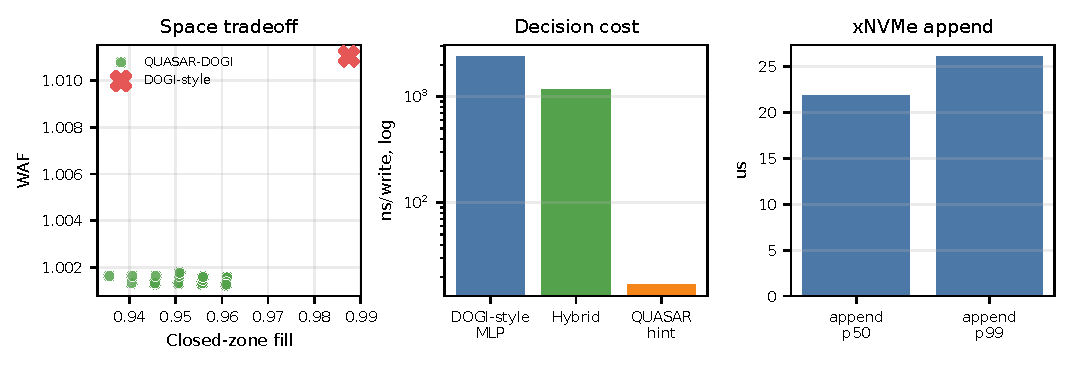
\includegraphics[width=0.88\textwidth]{../artifacts/figures/fast-style/fig4-resource-overhead.pdf}
\caption{Resource and overhead controls.  \system-\dogi bounds the closed-zone fill cost while removing stale secrets, the hint-routing decision path is orders of magnitude cheaper than the \dogi-style policy-decision microbenchmark, and xNVMe confirms a lower-overhead append command path than the zonefs helper used for full-suite replay accounting.}
\label{fig:resource-overhead}
\end{figure*}

\subsection{Robustness to Bad Hints and Stragglers}

The hardest \system cases are not clean epochs; they are wrong or missing hints, many tenants, and delayed-expiry stragglers.  On YCSB-A p4000, the clean hybrid has WAF 1.0000, zero stale secrets, and 28 semantic resets.  With 5\% missing hints, WAF remains 1.0000 but 3,361 stale secret blocks appear because some secret writes fall back to nonsemantic placement.  With 5\% wrong epochs, this trace still ends with zero stale secrets but increases reset activity to 112 resets.  With 5\% stragglers, exact secret-group packing can exceed the device open-zone budget; epoch-bin fallback completes within the budget but leaves waiting secrets, while epoch-bin plus residual migration reaches zero waiting at WAF 1.7098 after copying 234,549 residual blocks.

The residual fallback frontier shows why strict exposure mode cannot be the default.  Exchange-like and Sysbench-like representatives can reach zero final secret waiting with physical WAF 1.0182 and 1.2161, respectively.  YCSB-F p8000 reaches strict zero waiting only at physical WAF 3.5535 after migrating 1,168,095 residual blocks.  \system therefore exposes low-overhead, balanced, and strict-zero-wait profiles rather than hiding this tradeoff behind a single policy.

\begin{figure*}[t]
\centering
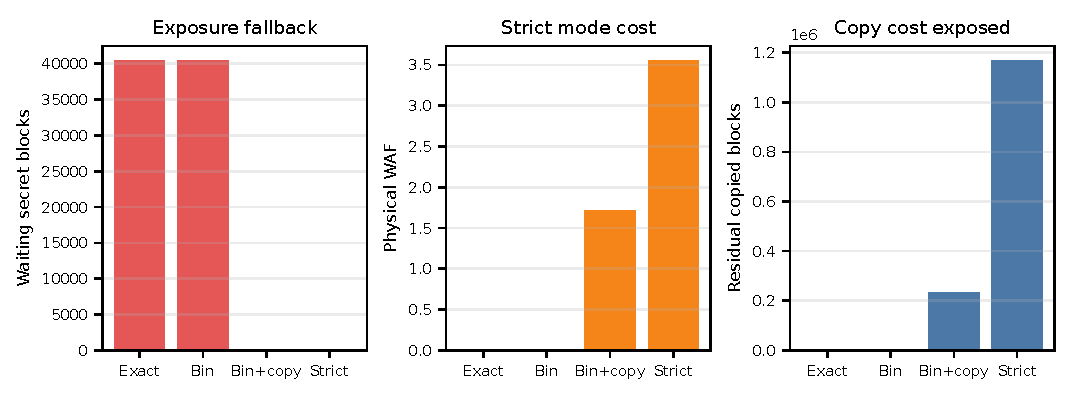
\includegraphics[width=0.88\textwidth]{../artifacts/figures/fast-style/fig6-robustness.pdf}
\caption{Robustness frontier.  Exact and binned placement can leave straggler secrets waiting under tight active-zone budgets.  Residual migration removes the exposure but increases physical WAF and copied blocks; strict zero-wait mode is therefore a policy point, not the default.}
\label{fig:robustness}
\end{figure*}

\subsection{Security Boundary}

The physical device advertises crypto-erase and block-erase sanitize support.  We executed crypto-erase sanitize and observed successful completion in the sanitize log.  This supports a deployment path where \system triggers hardware erase semantics at epoch boundaries.  The default result remains more conservative: \system reduces stale-secret exposure by aligning secret lifetime with reset eligibility, while physical erasure requires explicit sanitize or equivalent hardware support.  We do not use sanitize timing to claim foreground service latency: sanitize policy, batching, and SLO integration are deployment choices beyond the same-path placement comparison.

\subsection{Reproducibility}

The artifact manifest records 37 evidence artifacts, their roles, abbreviated hashes, and regeneration commands.  Validation finds zero hash mismatches, and the local acceptance report passes 41 of 41 gates.  These checks make the scoped evidence auditable.

\clearpage
\section{Related Work}

\noindent\textbf{Learned and heuristic placement for log-structured storage.}
\sepbit, \midas, and \dogi improve log-structured placement by predicting or adapting to invalidation behavior~\cite{sepbit,midas,dogi}.  \sepbit separates blocks by inferred invalidation time, \midas adapts group sizes and counts to workload dynamics, and \dogi uses oracle-guided analysis to motivate hot filtering, learned lifetime prediction, GC relocation policy, and dynamic group organization.  These systems are the right comparison class for \system because they represent the strongest storage-history view of placement.

\system is not an argument that learned placement is generally unnecessary.  For ordinary payload and workloads whose lifetime is not visible to the application, history is the right signal and \dogi-style placement can outperform semantic grouping.  \system targets a narrower regime where lifetime is not hidden from the software stack: a KEM artifact, ephemeral secret, or KMS envelope dies because a protocol epoch closes.  In that regime, prediction spends work approximating a label that the application already has, and a misplacement can leave expired secret bytes in a long-lived zone.

\noindent\textbf{Zoned storage and host-guided placement.}
\zns and related host-managed SSD interfaces expose placement and reclaim decisions to the host~\cite{zns,zenfs,xnvme}.  Systems such as ZenFS show how a host-side stack can map application writes onto zone append and reset operations.  \system builds on this host-managed direction but changes the placement key: instead of grouping only by hotness, stream, or predicted invalidation time, it groups secret-bearing writes by protocol death cohort.

Flexible Data Placement provides a different host-guided interface without forcing a full \zns software stack~\cite{fdp}.  \system can target native \zns by choosing zone families directly, or FDP-like devices by mapping intent and epoch to placement handles.  This makes \system a semantic placement policy rather than a device-specific API proposal.

\noindent\textbf{Benchmarks and trace methodology.}
FAST storage papers typically evaluate both synthetic controls and macro workloads.  DOGI uses FIO Zipf, YCSB-A/F, Varmail, Alibaba, and Exchange-like traces; our workload plan preserves these axes and adds PQC lifecycle overlays.  FIO, YCSB, and Sysbench remain important because they provide recognizable hot/cold, update-heavy, and DB-style pressure points~\cite{fio,ycsb,sysbench}.  The paper therefore treats pure PQC epoch streams only as sanity checks and uses DOGI/FAST-shaped pressure rows for headline claims.

\noindent\textbf{Post-quantum systems.}
Open Quantum Safe, liboqs, and oqs-provider provide software paths for deploying post-quantum algorithms in applications and TLS stacks~\cite{liboqs,oqsprovider}.  NIST's ML-KEM and ML-DSA standards make these deployments concrete targets rather than hypothetical future algorithms~\cite{nist-fips203,nist-fips204}.  Most systems work around PQC focuses on cryptographic correctness, interoperability, CPU overhead, and network handshake cost.  \system instead studies a storage side effect: lifecycle-heavy cryptographic metadata creates a placement signal that the block layer and device do not naturally observe.

\noindent\textbf{Secure erase and sanitization.}
Storage sanitization and crypto-erase mechanisms provide device-specific ways to destroy data or keys~\cite{nvme-sanitize}.  \system does not replace these mechanisms and does not claim that zone reset alone physically erases NAND.  It solves a placement precondition for secure disposal: expired secrets are isolated into zone families that can be reset or sanitized at the protocol boundary.  When hardware provides crypto-erase or sanitize semantics, \system gives the storage stack a deterministic point at which to trigger them.

\section{Discussion and Limitations}

\noindent\textbf{QUASAR is not a universal WAF optimizer.}
Easy rows deliberately show \dogi-style WAF near 1.0; there, \system's benefit is exposure reduction.  The scoped claim is that PQC death cohorts are invisible to history-based placement and become costly under pressure, not that \system wins every trace.

\noindent\textbf{Correctness, trust, and tenancy.}
Wrong or missing hints must not cause data loss: \system resets only after epoch-close confirmation; otherwise it migrates residuals, downgrades to normal GC, or sends low-confidence writes to overflow.  High-priority secret placement is emitted by trusted TLS/KMS/logging or policy components, with opaque cohort IDs, tenant-local namespaces, quotas, and admission limits to prevent priority inflation.

\noindent\textbf{Resource tradeoffs are explicit.}
Dedicated epoch zones can waste space, and strict zero-wait residual handling can be expensive on hostile rows such as YCSB-F p8000.  The default hybrid reserves exact placement for high-security cohorts, bins sparse cohorts, sends uncertain writes to overflow, and makes strict tenant/residual modes opt-in.

\noindent\textbf{Device and deployment boundaries.}
Zone reset alone is not physical NAND erasure; strong erasure requires sanitize or hardware crypto-erase, with deployment-specific scheduling cost.  The physical evidence uses one WD ZN540-class device, zonefs replay, liboqs/OpenSSL traces, a TLS socket trace, and an xNVMe probe.  Exact DOGI/MiDAS/SepBIT runs stay separate because their units differ from packed actual-\zns replay.  We report host-visible resets/utilization, but not internal wear telemetry or full SPDK poll-mode replay.

\section{Conclusion}

Post-quantum services can write KEM artifacts, bounded secret-bearing records, signatures, metadata, and payload together, but these objects die for different protocol reasons.  \system exposes that lifecycle signal as a small placement hint, keeps \dogi-style history placement for payload, and packs short-lived PQC objects by death cohort.  Actual-\zns experiments support the scoped claim: \system removes stale-secret exposure across PQC overlays and reduces GC/WAF when pressure makes mixed cohorts expensive.


\bibliographystyle{abbrv}
\bibliography{ref}

\end{document}
